\documentclass[12pt, letterpaper]{article}
\usepackage{graphicx}
\usepackage{tabularx}
\usepackage{pgfplots}
\pgfplotsset{width=10cm}

\title{NLP Twitter Analysis}
\author{Hamed Feizabadi}
\date{var-date}

\begin{document}
\maketitle

\section{Introduction}
Our source for this project is Twitter. You should create a file named "users.csv" inside src folder which contains the Twitter username, University name an Actual name of the users you wish to analyze.

\section{Data Collection}
We used selenium $>=$ 4.6.0 for collecting data from Twitter. This tool helps us to bring up an actual browser and navigate through the pages. Note that you should have Chrome installed on your system for this to work. Then you can simply install other dependencies form pyproject.toml file using poetry or other package managers.
The crawler script reads the users.csv file and for each user, it navigates to the user's profile and collects the tweets. The tweets are stored in a file named unlabeled.db inside data\slash raw folder. Then labeling script uses this and with the help of ChatGPT model, it generates the labels for each tweet and stores them in data\slash raw\slash labeled-run-date.csv file.

\section{Data Format}
The data is stored in a csv file with the following format: tweet\_time, tweet\_owner, tweet\_text, owner\_university, owner\_name, label.
We use tweet\_time, tweet\_owner as unique identifiers for each tweet. The tweet\_owner is Twitter username of the owner. The tweet\_text is the actual text of the tweet. owner\_university and owner\_name are the university and actual name of the tweet owner. The label is the generated label for the tweet.

\section{Data Preprocessing}
We have splitted data with three criteria: split by sentence with hazm sentence tokenizer, split by word with hazm word tokenizer, split by word with hazm lemmatizer.

For cleaning the data, we used the following steps: replace emojis, remove urls, remove hashtags, remove mentions, remove numbers, remove punctuations. We used the hazm and nltk libraries for this purpose.

\section{Labeling}
We give label to the whole tweet using ChatGPT. For more info about labeling see the src\slash utils\slash label.py file.

\section{Statistics}
\begin{center}
\begin{tabular}{ |c|c|c|c| } 
    \hline
    tweet count & sentence count & word count & unique word count \\ 
    \hline
    var-tweet-count & var-sentence-count & var-word-count & var-unique-word-count \\
    \hline
\end{tabular}
\end{center}

\begin{center}
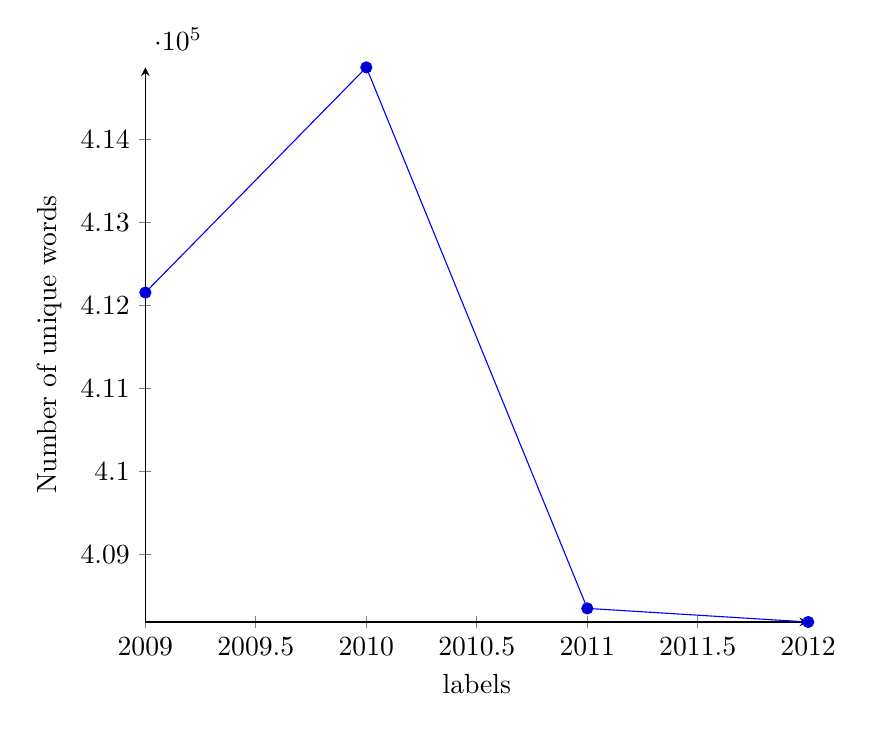
\begin{tikzpicture}
\begin{axis}[
    axis lines=left, 
    xlabel=labels, 
    ylabel=Number of unique words,
    x tick label style={
		/pgf/number format/1000 sep=}
]
\addplot 
	coordinates {(2012,408184) (2011,408348)
		 (2010,414870) (2009,412156)};
\end{axis}
\end{tikzpicture}
\end{center}

\end{document}
